%!TEX program = xelatex
\documentclass[11pt]{beamer}

\usepackage{amsfonts}
\usepackage{amsmath}
\usepackage{blindtext}
\usepackage{enumitem}

\usepackage{amsfonts}
\usepackage{amsmath}
\usepackage{amssymb}
\usepackage{blindtext}
\usepackage{enumitem}
\usepackage{fancyvrb}

\usetheme{SaoPaulo}

\title{Python Basics!}
\subtitle{strings, functions, scope}
\author{CS101 Lecture \#4}
\date{2016-10-10}

\setcounter{showSlideNumbers}{1}

\begin{document}
  \setcounter{showProgressBar}{0}
  \setcounter{showSlideNumbers}{0}

%%%%%%%%%%%%%%%%%%%%%%%%%%%%%%%%%%%%%%%%%%%%%%%%%%%%%%%%%%%%%%%%%%%%%%%%%%%%%%%%
\frame{\titlepage}

%%%%%%%%%%%%%%%%%%%%%%%%%%%%%%%%%%%%%%%%%%%%%%%%%%%%%%%%%%%%%%%%%%%%%%%%%%%%%%%%
\setcounter{framenumber}{0}
\setcounter{showProgressBar}{1}
\setcounter{showSlideNumbers}{1}

%%%%%%%%%%%%%%%%%%%%%%%%%%%%%%%%%%%%%%%%%%%%%%%%%%%%%%%%%%%%%%%%%%%%%%%%%%%%%%%%
\section{Administrivia}

%%%%%%%%%%%%%%%%%%%%%%%%%%%%%%%%%%%%%%%%%%%%%%%%%%%%%%%%%%%%%%%%%%%%%%%%%%%%%%%%
\begin{frame}
  \frametitle{Administrivia}
  \Enlarge
  \begin{itemize}
%  \myitem  Register your i>clickers on the course Compass page---attendance counts from today! \pause
%    \begin{itemize}
%    \mysubitem  Don't panic! \pause
%    \end{itemize}
%  \myitem  Complete Homework \#1 before 6:00 p.m. today. \pause
  \myitem  Homework \#2 is due Tuesday Oct.\ 3. 
  %\pause
%  \myitem  No lab next week (Labor Day).
  \end{itemize}
\end{frame}


%%%%%%%%%%%%%%%%%%%%%%%%%%%%%%%%%%%%%%%%%%%%%%%%%%%%%%%%%%%%%%%%%%%%%%%%%%%%%%%%
\section{Data Types---Strings}

%%%%%%%%%%%%%%%%%%%%%%%%%%%%%%%%%%%%%%%%%%%%%%%%%%%%%%%%%%%%%%%%%%%%%%%%%%%%%%%%
\begin{frame}
  \frametitle{ASCII table}
  \Enlarge
  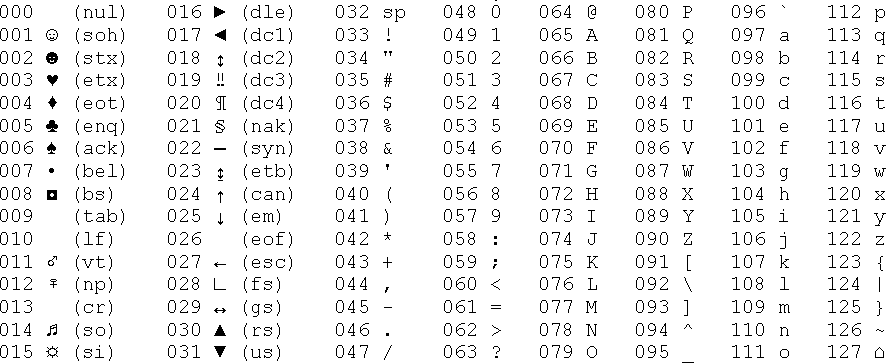
\includegraphics[width=\textwidth]{./img/ascii-table.png} \\ \pause
  
  {\small The table provides an \emph{encoding} scheme from symbols to numbers} \\
  \texttt{72 69 76 76 79} = \texttt{H E L L O} %\pause
  
  %\texttt{'HELLO'}
\end{frame}

%%%%%%%%%%%%%%%%%%%%%%%%%%%%%%%%%%%%%%%%%%%%%%%%%%%%%%%%%%%%%%%%%%%%%%%%%%%%%%%%
\begin{frame}
  \frametitle{How to store text on computer?}
  \Enlarge

  \begin{itemize}
  \myitem \texttt{H E L L O} = \texttt{72 69 76 76 79} \pause
  \myitem  Each symbol is stored individually, one byte long: \\
   \vspace{2mm} \pause
    \begin{tabular}{*{27}{l}}
      72 & \texttt{01001000} \\
      69 & \texttt{01000101} \\
      76 & \texttt{01001100} \\
      76 & \texttt{01001100} \\
      79 & \texttt{01001111} \\
    \end{tabular} \pause
    
    \vspace{2mm}
    {\small \texttt{'HELLO'} : \textcolor{CS101GradBot}{\texttt{01001000 01000101 01001100 01001100 01001111}}}
  \end{itemize}
\end{frame}


%%%%%%%%%%%%%%%%%%%%%%%%%%%%%%%%%%%%%%%%%%%%%%%%%%%%%%%%%%%%%%%%%%%%%%%%%%%%%%%%
\begin{frame}
  \frametitle{Strings}
  \Enlarge

  \begin{itemize}
  \myitem  As a literal:  text surrounded by quotes.
    \begin{itemize}
    \mysubitem  \texttt{'DEEP'}, or \texttt{"DEEP"} \pause
    \mysubitem single quote(\texttt{''}) and double quote (\texttt{""}) are equivalent (not in C or C++)
    \end{itemize}\pause
  \myitem  Can have arbitrary length, including an empty string (\texttt{''}). \pause
  \myitem  Each unit is a character --- also a string type \pause
  \myitem  In C/C++, a character (`char') is a different data type from a string (`str')
  \end{itemize}
\end{frame}


%%%%%%%%%%%%%%%%%%%%%%%%%%%%%%%%%%%%%%%%%%%%%%%%%%%%%%%%%%%%%%%%%%%%%%%%%%%%%%%%
\begin{frame}
  \frametitle{String operations}
  \Enlarge

  \begin{itemize}
  \myitem  \textbf{Concatenation}:  combine two strings
    \begin{itemize}
    \mysubitem  Uses the \texttt{+} symbol (operator for string concatenation) \pause
    \mysubitem  \texttt{'RACE' + 'CAR'}\pause
    \mysubitem the ``same'' operator works differently with different types of operand (\emph{operator overload})
    \end{itemize}
  \end{itemize} \pause
   \vspace{-1mm}
   \hspace{15mm}\texttt{\textcolor{CS101GradBot}{1 + 2 = 3}} \\ \vspace{1mm}
   \hspace{15mm}\texttt{\textcolor{CS101GradBot}{'RACE' + 'CAR' = 'RACECAR'}} 
\end{frame}


%%%%%%%%%%%%%%%%%%%%%%%%%%%%%%%%%%%%%%%%%%%%%%%%%%%%%%%%%%%%%%%%%%%%%%%%%%%%%%%%
\begin{frame}
  \frametitle{String operations}
  \Enlarge

  \begin{itemize}
  \myitem  \textbf{Repetition}:  repeat a string
    \begin{itemize}
    \mysubitem  Uses the \texttt{*}
    \mysubitem  \texttt{'HELLO '*10}
    \end{itemize}
  \end{itemize}
\end{frame}


%%%%%%%%%%%%%%%%%%%%%%%%%%%%%%%%%%%%%%%%%%%%%%%%%%%%%%%%%%%%%%%%%%%%%%%%%%%%%%%%
\begin{frame}[fragile]
  \frametitle{String operations}
  \Enlarge

  \begin{itemize}
  \myitem  \textbf{Formatting}: Creates string with other data types inserted in \pause
    \begin{itemize}
    \mysubitem  Formats different data types as a string \pause
    \mysubitem  Requires a special indicator of Formatting: \texttt{\%}
    \mysubitem  Requires indicator of data type
    \end{itemize} \pause
  \begin{semiverbatim}
x = 123 * 54
s = "The value of x is: %\textcolor{CS101GradBot}{i}" % \textcolor{CS101GradBot}{x}
print(s)
  \end{semiverbatim}
  \end{itemize}
\end{frame}


%%%%%%%%%%%%%%%%%%%%%%%%%%%%%%%%%%%%%%%%%%%%%%%%%%%%%%%%%%%%%%%%%%%%%%%%%%%%%%%%
\begin{frame}
  \frametitle{Formatting operator}
  \Enlarge

  \begin{itemize}
  \myitem  Creates string with value inserted
    \begin{itemize}
    \mysubitem  Formats nicely
    \mysubitem  Requires indicator of type inside of string
      \begin{tabular}{*{27}{ll}}
        \texttt{'\%i'} & \texttt{int} \\
        \texttt{'\%f'} & \texttt{float} \\
        \texttt{'\%e'} & \texttt{float} (scientific notation) \\
        \texttt{'\%s'} & \texttt{str}
      \end{tabular}
    \end{itemize}
  \end{itemize}
\end{frame}

%%%%%%%%%%%%%%%%%%%%%%%%%%%%%%%%%%%%%%%%%%%%%%%%%%%%%%%%%%%%%%%%%%%%%%%%%%%%%%%%
\begin{frame}[fragile]
  \frametitle{Example}
  \Enlarge

  \begin{semiverbatim}
print( 'An integer:  \%i' \% 7 )
print( 'A float:     \%f' \% 7.0 )
print( 'A float:     \%e' \% 7.0 )
print( 'A string:    \%s' \% 'seven' )
  \end{semiverbatim}
\end{frame}

%%%%%%%%%%%%%%%%%%%%%%%%%%%%%%%%%%%%%%%%%%%%%%%%%%%%%%%%%%%%%%%%%%%%%%%%%%%%%%%%
\begin{frame}[fragile]
  \frametitle{Example}
  \Enlarge

  \begin{Verbatim}[commandchars=\\\{\}]
name = "Tao"
grade = 2 / 3
m1 = "Hello, %s!" % name
m2 = "Your grade is:  %f." % grade
print(m1)
print(m2) \pause

\textcolor{CS101PureBase}{
Hello, Tao!}
\textcolor{CS101PureBase}{
Your grade is 0.666667.} 
\end{Verbatim}

\iffalse
\begin{Verbatim}[commandchars=\\\{\}]
m3 = "Your grade is:  %\textcolor{red}{.3}f" % grade
print(m3) \pause

\textcolor{CS101PureBase}{
Your grade is 0.667.}
\end{Verbatim}
\fi

\end{frame} 

%%%%%%%%%%%%%%%%%%%%%%%%%%%%%%%%%%%%%%%%%%%%%%%%%%%%%%%%%%%%%%%%%%%%%%%%%%%%%%%%
\begin{frame}[fragile]
  \frametitle{Example}
  \Enlarge

  \begin{semiverbatim}
x = 3
s = ("%i" % (x+1)) * x**(5%x)
print(s)
  \end{semiverbatim}

  What does this program print?
  \begin{enumerate}[label=\Alph*]
  \item  \texttt{333333333333}
  \item  \texttt{444444444}
  \item  \texttt{9999}
  \item  \texttt{\%i\%i\%i\%i\%i}
  \end{enumerate}
\end{frame}


%%%%%%%%%%%%%%%%%%%%%%%%%%%%%%%%%%%%%%%%%%%%%%%%%%%%%%%%%%%%%%%%%%%%%%%%%%%%%%%%
\begin{frame}
  \frametitle{Special characters}
  \Enlarge

  \begin{itemize}
  \myitem  Special characters, start with \texttt{\textbackslash}
    \begin{tabular}{*{27}{l}}
      \texttt{\textbackslash n} & new line \\
      \texttt{\textbackslash t} & tab (tabular key)\\
      \texttt{\textbackslash \textbackslash} & \texttt{\textbackslash} \\
      \texttt{\textbackslash '} & \texttt{'} \\
      \texttt{\textbackslash "} & \texttt{"} \\
   \end{tabular} 
  \myitem \texttt{\textbackslash} is called the \emph{escape} character
  \begin{itemize}
  	\mysubitem  \textcolor{blue}{\small \texttt{\url{https://docs.python.org/2.0/ref/strings.html}}} 
  \end{itemize}
  \end{itemize}
  
\end{frame}


%%%%%%%%%%%%%%%%%%%%%%%%%%%%%%%%%%%%%%%%%%%%%%%%%%%%%%%%%%%%%%%%%%%%%%%%%%%%%%%%
\begin{frame}[fragile]
  \frametitle{Example}
  \Enlarge

  \hspace{10mm}Try: \\
  \hspace{12mm}\texttt{\small print('Hello Tao\texttt{\textcolor{red}{\textbackslash n}}Your grade is 0.667') \\
  \hspace{12mm}print('3 plus 5 is:\texttt{\textcolor{red}{\textbackslash t}}\%i', \% (3+5)) \\
  \hspace{12mm}print('put .ipynb file in: C:\texttt{\textcolor{red}{\textbackslash \textbackslash}}Users\texttt{\textcolor{red}{\textbackslash \textbackslash}}nick')
  }
\end{frame}

%%%%%%%%%%%%%%%%%%%%%%%%%%%%%%%%%%%%%%%%%%%%%%%%%%%%%%%%%%%%%%%%%%%%%%%%%%%%%%%%
\begin{frame}
  \frametitle{Quote in Quote}
  \Enlarge

  \begin{itemize}
  \myitem  ``Emily's not coming today''
  	\begin{itemize}
	\mysubitem try: \texttt{{\small print('Emily's not coming today')}}
	\mysubitem try: \texttt{{\small print("Emily's not coming today")}}
	\end{itemize}\pause
  \myitem ``Movie of the week is ''Beauty and Beast''''
  	\begin{itemize}
	\mysubitem \texttt{{\small print('Movie of the week is ''Beauty and Beast"')}}
	\mysubitem \texttt{{\small print("Movie of the week is ''Beauty and Beast" ")}}
	\end{itemize} \pause
  \myitem rule-of-thumb 
  	\begin{itemize}
	\mysubitem use double quote to enclose single quote
	\mysubitem use single quote to enclose double quote \pause
	\mysubitem use \texttt{\textbackslash '} or \texttt{\textbackslash "} for quotes inside a string \pause
	\mysubitem sometimes use triple quote (\texttt{''' '''})
	\end{itemize}
 \end{itemize}
\end{frame}


%%%%%%%%%%%%%%%%%%%%%%%%%%%%%%%%%%%%%%%%%%%%%%%%%%%%%%%%%%%%%%%%%%%%%%%%%%%%%%%%
\begin{frame}[fragile]
  \frametitle{Indexing operator \textbf{[]}}
  \Enlarge

  \begin{itemize}
  \myitem  Extracts single character
\begin{semiverbatim}
a = "FIRE"
a[0]
\end{semiverbatim}
  \myitem  The integer is the index. \pause
  \myitem  \textcolor{red}{We count from zero!} \pause
  \myitem  If negative, counts down from end. \pause
  \myitem  Does this work on other data types like \texttt{int}?
  \end{itemize}
\end{frame}

%%%%%%%%%%%%%%%%%%%%%%%%%%%%%%%%%%%%%%%%%%%%%%%%%%%%%%%%%%%%%%%%%%%%%%%%%%%%%%%%
\begin{frame}[fragile]
  \frametitle{Slicing operator \textbf{:}}
  \Enlarge

  \begin{itemize}
  \myitem  Extracts range of characters (\emph{substring}) \pause
  \myitem  Range specified inside of indexing operator \pause
\begin{semiverbatim}
a = "FIREHOUSE"
a[0:4]
\end{semiverbatim} \pause
  \myitem  Can be a bit tricky at first:
    \begin{itemize}
    \mysubitem  Includes character at first index
    \mysubitem  Excludes character at last index
    \end{itemize}
  \end{itemize}
\end{frame}

%%%%%%%%%%%%%%%%%%%%%%%%%%%%%%%%%%%%%%%%%%%%%%%%%%%%%%%%%%%%%%%%%%%%%%%%%%%%%%%%
\begin{frame}[fragile]
  \frametitle{Example}
  \Enlarge

  \begin{semiverbatim}
alpha = "ABCDE"
x = alpha[1:3]
  \end{semiverbatim}
  What is the value of \texttt{x}?
  \begin{enumerate}[label=\Alph*]
  \item  \texttt{'AB'}
  \item  \texttt{'ABC'}
  \item  \texttt{'BC'}
  \item  \texttt{'BCD'}
  \item  \texttt{'CD'}
  \end{enumerate}
\end{frame}

%%%%%%%%%%%%%%%%%%%%%%%%%%%%%%%%%%%%%%%%%%%%%%%%%%%%%%%%%%%%%%%%%%%%%%%%%%%%%%%%
\begin{frame}[fragile]
  \frametitle{Slicing operator \textbf{:} with stepsize}
  \Enlarge

  \begin{itemize}
  \myitem  Extracts a sub-range of characters with a \emph{stepsize}\pause
\begin{semiverbatim}
alpha = "ABCDE"  
alpha[1:3:\textcolor{CS101GradBot}{2}]   \hspace{2mm} \textcolor{CS101GradBot}{\small #last value is stepsize} \pause
'B'
\end{semiverbatim} \pause
\myitem Stepsize can be negative
\begin{semiverbatim}
alpha[4:1:\textcolor{CS101GradBot}{-1}] \pause
'EDC' \pause
alpha[-1:1:\textcolor{CS101GradBot}{-2}]
\end{semiverbatim}
  \end{itemize}
\end{frame}


%%%%%%%%%%%%%%%%%%%%%%%%%%%%%%%%%%%%%%%%%%%%%%%%%%%%%%%%%%%%%%%%%%%%%%%%%%%%%%%%
\section{Functions}

%%%%%%%%%%%%%%%%%%%%%%%%%%%%%%%%%%%%%%%%%%%%%%%%%%%%%%%%%%%%%%%%%%%%%%%%%%%%%%%%
\begin{frame}
  \frametitle{And now for something different...}
  \Enlarge

  \begin{itemize}
  \myitem  A \emph{function} is a small program (block of code) we can run within Python. \pause
    \begin{itemize}
    \mysubitem  Saves us from rewriting code
    \mysubitem  Don't reinvent the wheel!
    \end{itemize} \pause
  \myitem  Analogy:  Functions are more verbs. \pause
  \myitem  Also called subroutine or procedure.
  \end{itemize}
\end{frame}

%%%%%%%%%%%%%%%%%%%%%%%%%%%%%%%%%%%%%%%%%%%%%%%%%%%%%%%%%%%%%%%%%%%%%%%%%%%%%%%%
\begin{frame}
  \frametitle{Function calls}
  \Enlarge

  \begin{itemize}
  \myitem  When we want to execute a function, we call or invoke it. \pause
  \myitem  Use name of the function with parentheses. \pause
    \begin{itemize}
    \mysubitem  \texttt{print()}
    \end{itemize} \pause
  \myitem  Many functions come built-in to Python or in the standard library. \pause
  \myitem  Others we will compose at need.
  \end{itemize}
\end{frame}

%%%%%%%%%%%%%%%%%%%%%%%%%%%%%%%%%%%%%%%%%%%%%%%%%%%%%%%%%%%%%%%%%%%%%%%%%%%%%%%%
\begin{frame}
  \frametitle{Arguments}
  \Enlarge

  \begin{itemize}
  \myitem  Functions can act on data. \pause
  \myitem  \emph{Arguments} are the input to functions. \pause
  \myitem  Functions can return a value.  (fruitful) \pause
  \myitem  Return values are the output of a function. \pause
    \begin{itemize}
    \mysubitem  \texttt{print('10')} \pause
    \mysubitem  \texttt{len('Rex Kwon Do')} \pause
    \mysubitem  \texttt{abs(-123)}
    \end{itemize}
  \end{itemize}
\end{frame}

%%%%%%%%%%%%%%%%%%%%%%%%%%%%%%%%%%%%%%%%%%%%%%%%%%%%%%%%%%%%%%%%%%%%%%%%%%%%%%%%
\begin{frame}
  \frametitle{Arguments}
  \Enlarge

  \begin{itemize}
  \myitem  \emph{Arguments} are values passed \emph{to} a function. \pause
  \myitem  A function can accept zero to many arguments. \pause
  \myitem  Multiple arguments are separated by commas:
    \begin{itemize}
    \mysubitem  \texttt{min( 1,4,5 )}
    \mysubitem  \texttt{max( 1,4,5 )}
    \end{itemize}
  \end{itemize}
\end{frame}

%%%%%%%%%%%%%%%%%%%%%%%%%%%%%%%%%%%%%%%%%%%%%%%%%%%%%%%%%%%%%%%%%%%%%%%%%%%%%%%%
\begin{frame}
  \frametitle{Type conversion.}
  \Enlarge

  \begin{itemize}
  \myitem  A set of built-in functions to convert data from one type to another. \pause
    \begin{itemize}
    \mysubitem  \texttt{float( "0.3" )}
    \mysubitem  \texttt{str( 3 + 5j )}
    \end{itemize} \pause
  \myitem  Be careful of nonsense:
    \begin{itemize}
    \mysubitem  \texttt{int( "Rex" )}
    \mysubitem  \texttt{int( 3 + 5j )}
    \end{itemize}
  \end{itemize}
\end{frame}

%%%%%%%%%%%%%%%%%%%%%%%%%%%%%%%%%%%%%%%%%%%%%%%%%%%%%%%%%%%%%%%%%%%%%%%%%%%%%%%%
\begin{frame}
  \frametitle{User input}
  \Enlarge

  \begin{itemize}
  \myitem  \texttt{input()} is a built-in function. \pause
  \myitem  Takes keyboard input from prompt by user \pause
  \myitem  No argument to the function \pause
  \myitem  Return value:  keyboard input from user (as \texttt{str})
  \end{itemize}
\end{frame}

%%%%%%%%%%%%%%%%%%%%%%%%%%%%%%%%%%%%%%%%%%%%%%%%%%%%%%%%%%%%%%%%%%%%%%%%%%%%%%%%
\begin{frame}
  \frametitle{Goal}
  \Enlarge

  \begin{itemize}
  \myitem  A program should achieve a goal. \pause
  \myitem  Next time we will write our first nontrivial program.
  \end{itemize}
\end{frame}

%%%%%%%%%%%%%%%%%%%%%%%%%%%%%%%%%%%%%%%%%%%%%%%%%%%%%%%%%%%%%%%%%%%%%%%%%%%%%%%%
\section{Reminders}

%%%%%%%%%%%%%%%%%%%%%%%%%%%%%%%%%%%%%%%%%%%%%%%%%%%%%%%%%%%%%%%%%%%%%%%%%%%%%%%%
\begin{frame}
  \frametitle{Reminders}
  \Enlarge

  \begin{itemize}
  \myitem Homework \#2 is due Wed Oct.\ 19. 
  \end{itemize}
\end{frame}

\end{document}
